\documentclass{article}
\usepackage[utf8]{inputenc}
\usepackage[margin=1in]{geometry}
\title{Assignment 1: HPSC}
\author{Manan Doshi}
\date{5 March 2018}
\usepackage{graphicx}

\begin{document}
\graphicspath{{/}}
\maketitle

\section{Introduction}
In this assignment, we evaluate the performance on Monte Carlo method and the Trapezoidal rule to evaluate \(\int_{0}^{1} \sin x \, dx \). The code for evaluating the integral via both methods lives in \texttt{utility.c}. Timing is done using the built-in time methods in \texttt{C}. \texttt{main.c} is the wrapper program to time and evaluate integrals using either of the methods in parallel.\\

Usage: \verb|./main method num_iterations num_points num_threads|\\
Example: \verb|./main `T' 2 1000 2|\\

For the timing study, multiple runs of single iterations were used (using a bash script, \texttt{main\_script.sh}) rather than one run with multiple iterations since the compiler seemed to be optimizing it's runs when the same code of looped over multiple runs. Time taken did not grow linearly with number of iterations when the iterations were done internally. Using the bash script, \texttt{main.c} is run multiple times and it's output is appended to \texttt{timing\_method.csv} after which a python script is run to compute averages and make plots.

\section{Convergence Study}
The following plots show the absolute error of both the methods with increasing number of points. It can be clearly seen that both the methods converge to the actual value of the integral(2.00). The Monte Carlo method is more `erratic' in it's convergence because of the stochasticity involved.

\begin{figure}[h!]
\centering
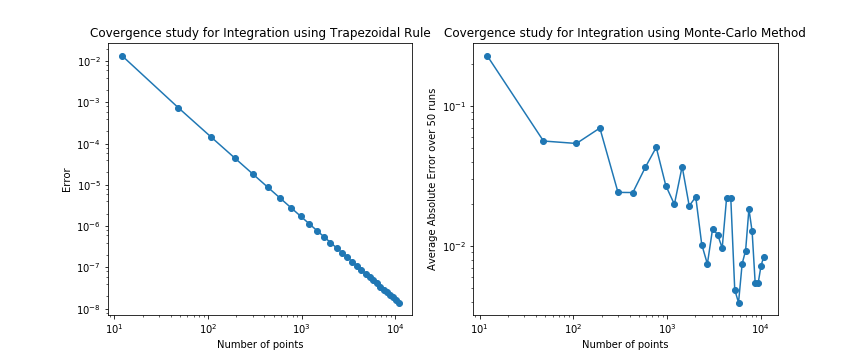
\includegraphics[scale=0.5]{conv}
\end{figure}

\newpage
\section{Timing Study}

Following are the log-log plots of the time taken for the code to run using various number of threads (Number of points = $100000$). It can be clearly seen that, for the trapezoidal rule, the time take decreases with the increase in the number of threads till 4 threads and then massively increases. The reason for this is that the machine has just $4$ processors and beyond that, the threads ave to be run on the same processor. The overhead due to scheduling and parallelizing substantially increase the time taken for the code to run.

The Monte Carlo method, on the other hand slows down with threading. This can perhaps be attributed to the generation of random numbers. Random numbers are generated using a pseudo random number generator, which, given a seed produces an array of random numbers sequentially. Every time a thread queries for a random number, it is probably computed in a serial fashion using the PRNG. Thus the code essentially remains serial and an increase in threads increases the time taken due to the overhead. 
\begin{figure}[h!]
\centering
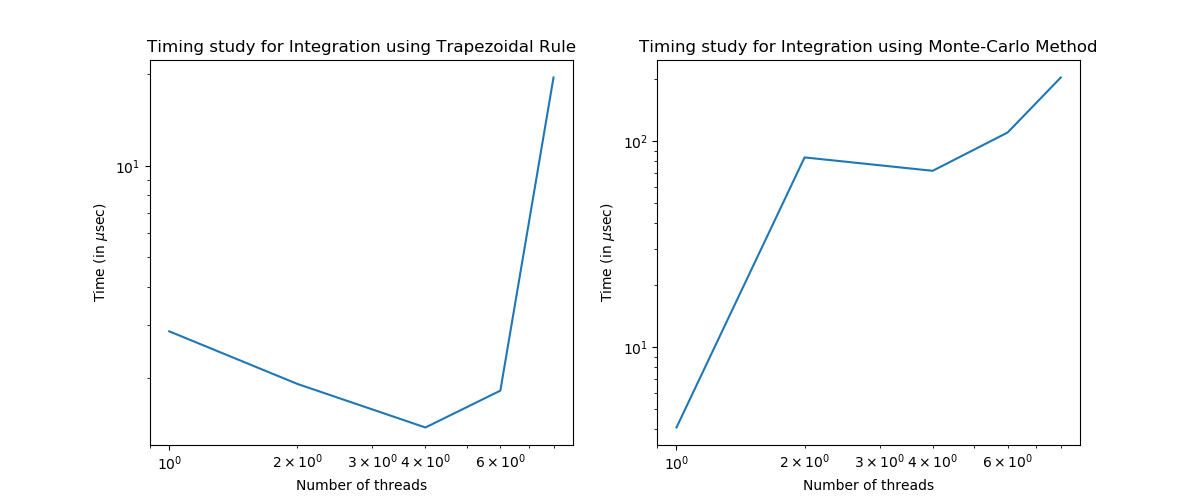
\includegraphics[scale=0.6]{timing}
\end{figure}

\end{document}
